\documentclass[12pt]{article}
\title{Edzőterem működését támogató szoftver PureScript és Vue.js alapokon}
\author{Mezei Botond, Szabó Benedek}
\date{2023}
\renewcommand{\contentsname}{Tartalomjegyzék}
\usepackage[utf8]{inputenc}
\usepackage{graphicx}
\graphicspath{ {./images/} }
\usepackage{wrapfig}
\renewcommand{\figurename}{Ábra}
\usepackage{amsmath}
\usepackage{subcaption}
\usepackage{amssymb}
\usepackage[export]{adjustbox}
\usepackage[magyar]{babel}
\usepackage[breaklinks]{hyperref}
\usepackage{microtype}
\usepackage[T1]{fontenc}
\usepackage{lmodern}
\usepackage{multirow}
\usepackage[table]{xcolor}
%\usepackage{natbib}

\setlength{\arrayrulewidth}{0.5mm}
\setlength{\tabcolsep}{7pt}
\renewcommand{\arraystretch}{2.5}

\textwidth=14cm \textheight=20cm
%\hoffset=-1cm
%\voffset=-1cm

\newtheorem{theorem}{Theorem}[section]
\newtheorem{acknowledgement}[theorem]{Acknowledgement}
\newtheorem{algorithm}[theorem]{Algorithm}
\newtheorem{axiom}[theorem]{Axiom}
\newtheorem{case}[theorem]{Case}
\newtheorem{claim}[theorem]{Claim}
\newtheorem{conclusion}[theorem]{Conclusion}
\newtheorem{condition}[theorem]{Condition}
\newtheorem{conjecture}[theorem]{Conjecture}
\newtheorem{corollary}[theorem]{Corollary}
\newtheorem{criterion}[theorem]{Criterion}
\newtheorem{definíció}[theorem]{Definíció}
\newtheorem{discussion}[theorem]{Discussion}
\newtheorem{example}[theorem]{Example}
\newtheorem{exercise}[theorem]{Exercise}
\newtheorem{explanation}[theorem]{Explanation}
\newtheorem{illustration}[theorem]{Illustration}
\newtheorem{lemma}[theorem]{Lemma}
\newtheorem{notation}[theorem]{Notation}
\newtheorem{problem}[theorem]{Problem}
\newtheorem{proposition}[theorem]{Proposition}
\newtheorem{remark}[theorem]{Remark}
\newtheorem{solution}[theorem]{Solution}
\newtheorem{summary}[theorem]{Summary}

\makeatletter
%\renewcommand*{\@biblabel}[1]{–}
\makeatother

\begin{document}
\begin{titlepage}

	\begin{center}
	\mbox{}\\
	\vspace{35mm}
	\huge
	\textsc{Diplomamunka}
	\end{center}

	
	\vspace{55mm}
	\Large
	\hspace*{\fill} 
	\textbf{Mezei Botond, Szabó Benedek}
	
	\begin{center}
	\vspace{55mm}
	Debrecen\\	
	2023
	
	\end{center}
\end{titlepage}
\begin{titlepage}

	\vspace*{-2cm}
	\hspace*{-1.5cm}

	\begin{center}
	\large
	Debreceni Egyetem
	
	Informatikai Kar	

	Számítógéptudományi Tanszék
	
	\vspace{17mm}
	\huge
	\LARGE
    \textbf{Edzőterem működését támogató szoftver PureScript és Vue.js alapokon}
	
	\vspace{15mm}
	\large
	\textsc{Diplomamunka}
	
	\normalsize
	\vspace{20mm}
	\textsc{Készítette:}
	
	\vspace{5mm}
	\Large
	\textbf{Mezei Botond és Szabó Benedek}
	
	\normalsize
	programtervező informatika szakos hallgatók
	
	\vspace{18mm}
	\textsc{Témavezető:}\\
	\vspace{5mm}
	\large
	Dr. Battyányi Péter \\
	\normalsize
	adjunktus\\
	
	\vspace{32mm}
	Debrecen\\	
	2023
	
	\end{center}
\end{titlepage}
\newpage
\tableofcontents
\newpage
\section*{Bevezetés}
\addcontentsline{toc}{section}{Bevezetés}

A funkcionális programozás egy kevésbé elterjedt programozási paradigma. Noha számos népszerű nyelv használ funkcionális elemeket \cite{Java} \cite{py} \cite{cpp},  a teljesen funkcionális fejlesztés nem annyira népszerű. Megismerése az oktatásban sem igazán hangsúlyos. Ennek ellenére számos előnnyel rendelkezik, melyeket a későbbi fejezetekben fogunk részletezni. Másfajta gondolkosámódot igényel, mint az imperatív megközelítés: a "hogyan?" helyett a "mit csináljon a program?" kérdésre adja meg a választ.

A dolgozatban tárgyalt szoftver backend komponensének elkészítésére a PureScript nyelvet választottuk. Ez egy tisztán funkcionális és erősen típusos programozási nyelv, mely Javascript-re fordul. Azért választottuk ezt a nyelvet, mert tisztán funkcionális, a közelmúltban megjelent nyelv, mely a többi funkcionális nyelvhez (Haskell, Elm) képest modernebb, erőteljesebb, könnyebben használható és teljesebb \cite{CS}.

Munkánk elsődleges célja egy edzőterem működését támogató szoftver elkészítése PureScript backend és Vue.js frontend használatával. Ezen felül szeretnénk megvizsgálni és bemutatni a funkcionális nyelvek használatának előnyeit és lehetőségeit leginkább webalkalmazások fejlesztése során. A szoftver elkészültét követően implementálásra kerül ugyanez a backend Java nyelven a Spring keretrendszer használatával. Célunk a két verzió sebességének és fejlesztési tapasztalatainak összehasonlítása.

A huszonegyedik században egy korszerű edzőteremnek szüksége van egy szoftverre, amely a mindennapi üzletmenetet támogatja. Választásunk azért erre a területre esett, mert egyrészt mindketten szeretünk edzeni járni, másrészt pedig a szoftver összetettsége már alkalmas lehet a PureScript nyelv megismerésére, lehetőségeinek és előnyeinek bemutatására, illetve egy elterjedtebb technológiával (Java, Spring) készült változatával való összehasonlításra.

Az alkalmazás felhasználói az edzőterem recepciós kollégái. A rendszerben lehetőség van rögzíteni:
\begin{itemize}
\item vendégeket
\item bérlettípusak (jegytípusokat)
\item a felhasználók jegyeit, bérleteit
\item öltözőszekrényeket
\end{itemize}

A\textit{Vendégek} oldalon listázhatjuk a regisztrált vendégeket, újat regisztrálhatunk, a meglévők adatait módosíthatjuk, vendéget törölhetünk. A vendégek számára bérleteket vagy jegyeket lehet vásárolni. A továbbiakban bérletnek nevezzük azt a tagásgot, ami egy időtartamra engedélyezi a terem használatát, jegynek pedig ami alkalmakhoz kötött. A jegyeknek is van egy elévülési ideje. Minden belépőnek három ára van: teljes, diák és klub ár. A felhasználóknak klubtagság vásárlására van lehetőségük, amely különböző előnyökkel jár, például kedvezőbb bérletárak.

A vezérlőpulton lehetőség van a vendégek beléptetésére: a regisztrált vendégek listájából ki kell választani az illetőt. A listában csak az aktív bérlettel vagy érvényes jeggyel rendelkezők jelennek meg. A illetőhöz hozzárendelődik a neme szerint egy szabad öltözőszekrény. Jeggyel rendelkező vendégek számára a jegyen található fennmaradó alkalmak száma eggyel csökken. Az öltözőszekrények megtekintésére egy külön lap szolgál. Itt nemek szerint meg lehet tekinteni minden szekrény állapotát, illetve az előzménytörténetét, vagyis mikor és ki használta. A foglalt szekrények piros színnel jelennek meg.

A vezérlőpulton  a beléptetett vendégek kijelentkeztetésére is van lehetőség. Ezt úgy tehetjük meg, hogy a feljövő listából kiválasztjuk az illetőt. Ilyenkor felszabadul a szekrénye. 

Minden oldal tetején egy navigációs sáv található, mellyel a megfelelő lapra ugorhatunk.

A közös munka során az egyik legnépszerűbb verziókezelő rendszert, a git-et használtuk a Github szolgáltatóval. Az extrém programozás módszerei közül többet is alkalmaztunk, például a páros programozást, mely hatékonynak bizonyult. Lényege, hogy az egyik fejlesztő írja a kódot, a másik pedig segíti közben.

\newpage
\section{Szakirodalmi áttekintés}

\subsection{Funkcionális programozás}
A funkcionális programozás egy programozási paradigma. Több programozási nyelv is tartozik ide, melyeket bizonyos tulajdonságok, módszereik, lehetőségeik, gondolkodási logikájuk köti össze. Az egyik korai funkcionális nyelv a Lisp, melyet John McCarthy alkotott meg az 1950-es évek végén \cite{JM}. Ismertebb funkcionális nyelvek például Haskell, Elm, Erlang, Scala vagy a PureScript. 
A funkcionális programozás során a fejlesztő azt specifikálja a programban, hogy mit kell kiszámítani, és nem azt, hogy hogyan, milyen lépésekben \cite{VD}. A program függvények hívásából és ezek kiértékeléséből áll, nincs értékadás, csak érték kiszámítás \cite{VD}. A függvényt leginkább úgy értjük, hogy egy leképezés egy adott halmazról egy másik halmazra\cite{sy}. A listák (vagy halmazok) kezelésének ezért kiemelt szerep jut a funkcionális nyelvekben. A program tartalmazhat a nyelvben előre definiált, és a programozó által definiált függvényeket. A függvények névvel és opcionálisan argumentumokkal rendelkeznek. Az előállított érték(ek) megegyező paraméterekkel mindig ugyanaz. A rekurzió egy nagyon gyakori koncepció funkcionális nyelvekben.

Egy másik nagy paradigma az imperatív programozás. Az imperatív nyelvek lényege, hogy a programozó a lépéseket definiálja a kódban, melyet a számítógépnek el kell végeznie (utasítások). A legismertebb imperatív nyelv a C.

A logikai programozási paradigma lényege, hogy a programozó állításokat, szabályokat rögzít, melyek használatával a gép automatikusan kikövetkezteti, hogy egy kérdéses állítás igaz, vagy sem. Ilyen nyelv például a Prolog.

Manapság az egyik legelterjedtebb paradigma az objektumorientált programozás. Ez egy gondolkodásmód, tervezési módszer is egyben. A valós világot osztályok formájára képezi le, melynek egyedeit objektumok személyesítenek meg. Legfőbb elvei az egységbezárás (encapsulation: az adatmodell és az eljárásmodell szétválaszthatatlansága), öröklődés (újrafelhasználhatóság kiterjesztése), hozzáférés-szabályozás és többalakúság (polimorphism: lehetővé teszi, hogy ugyanarra az üzenetre különböző objektumok a saját módjukon válaszoljanak) \cite{VD}.

A ma leginkább használatos nyelvekre általánosságban igaz az, hogy nem csupán egyetlen paradigmát követnek tisztán, hanem többet vegyítenek. Ennek az az oka, hogy minden paradigmának megvan a maga előnye (és persze hátránya is), és ezeket az előnyöket érdemes kihasználni. Például a Java (2023. áprilisában a harmadik legtöbbet használt nyelv \cite{TIO}) alapjaiban imperatív, objektumorientált, de a nyolcas verziótól kezdve \cite{Java} megjelennek benne funkcionális elemek, például a lambda kifejezések. A nyelv hivatalos oldala \cite{Java} "erőteljes kiterjesztés"-nek nevezi ezt a lépést.
A Java mellett több elterjedt, nem tisztán funkcionális nyelv, mint például a Python vagy a C++ is épít be funkcionális elemeket \cite{py} \cite{cpp}.

\subsubsection{A funkcionális programozás előnyei}
A funkcionális programozás, mint paradigma, számos előnnyel rendelkezik. Az imperatív gondolkodás kötöttségét egy másfajta megközelítéssel oldja fel. A lényeg, hogy \textit{mit} csináljon a program, és nem az, hogy \textit{hogyan}. Ez az ötlet a programozótól is  másfajta megközelítést, gondolkodásmódot kíván, és máshogy strukturált kódot is fog eredményezni. 

Ránézésre jobban érthető, átláthatóbb, esztétikusabb kód. A szoftver "viselkedése" jobban olvasható \cite{CS}. Ez az előny egyszerűen a funkcionális szintaktikából és gondolkodásmódból adódik. A következő Java kódrészletek Boris Radojicic 2022-es cikkéből \cite{sy} származnak. Az elsőn az iteratív megközelítés látható:

\begin{verbatim}
public List<String> getAddresses(List<Person> persons) {
    List<String> addresses = new ArrayList<>();
    for (int i = 0; i < persons.size(); i++) {
        Person person = persons.get(i);
        if (person.hasValidData()) {
            String address = person.getAddress();
            addresses.add(address.trim());
        }
    }
    return addresses;
}
\end{verbatim}
A következő kódrészlet pedig a funkcionális megközelítést alkalmazza:
\begin{verbatim}
public List<String> getAddresses(List<Person> persons) {
    return persons.stream()
            .filter(person -> person.hasValidData())
            .map(person -> person.getAddress())
            .map(address -> address.trim())
            .collect(Collectors.toList());
}
\end{verbatim}
Míg a két kód ugyanazt a viselkedést eredményezi, a kettőre ránézve elmondható, hogy a második olvashatóbb és tömörebb.

Nagy fokú újrafelhasználhatóság. Mivel egy funkcionális program gyakorlatilag függvények deklarálásából és függvényhívásokból áll, ezeket a függvényeket nagy mértékben újra lehet hasznosítani, elkerülve a feleslegesen duplikált kódrészleteket. A felesleges kód rontja az átláthatóságot és több erőforrást is igényel.

Könnyebb tesztelhetőség. Mivel a funkcionális programban nincsenek állapotok és mellékhatások, így könnyebb lefedni az összes esetet. Illetve ebből kifolyóan, a függvénynek bizonyos bemenő paraméterekre mindig ugyanazt az egyértelmű kimenetet kell előállítania.

A rekurzió hatékony használata. A rekurzió a funkcionális nyelvek gyakori eleme. Átláthatóvá és egyértelművé teszi a kódot teszi a kódot bizonyos problémák esetében, ahol a rekurzív definiálás a természetesebb megoldás. A rekurziónak egy speciális esete a farokrekurzió. Ez azt jelenti, hogy a rekurzív hívás a legutolsó művelet, amit a függvény végrehajt. Nagy előnye, hogy idő és erőforrás takarékos a nem farokrekurzív függvényekkel szemben, ugyanis a fordító kevesebb információt kell, hogy tároljon ilyen módon a veremben.

\subsubsection{A funkcionális programozás nehézségei}

Az előnyök között első helyen állt az átláthatóság és érthetőség. Ehhez viszont hozzátartozik az, hogy a fejlesztő előtte megismerje és elsajátítsa a funkcionális programozás gondolkodásmódját, ami néha bizony nem egyszerű és nem a legtermészetesebb megoldásnak tűnhet.

Memóriahasználat és teljesítmény. Mivel a funkcionális nyelvek nem használnak érték-átadást, sokszor egy változó értékének megváltozása helyett létrejön egy újabb, ami így több erőforrást igényel \cite{JN}. A legtöbb funkcionális nyelv ennek ellenére számos módon ígyekszik ezt kompenzálni: farokrekurzió, lusta kiértékelés, "smart linking". A több paradigmát támogató vagy OOP nyelvek nem feltétlen implementálják ezeket az optimalizációkat \cite{JN}.

Mivel a funkcionális nyelvek használata kevésbé elterjedt, kevesebb eszköz, keretrendszer áll rendelkezésre és kevesebb a felhasználók, szakértők száma.

\subsection{PureScript}

A PureScript egy erősen típusos, tisztán funkcionális nyelv. Javascript kódra fordul. Ennek előnye, hogy a kód írására egy szép, könnyen áttekinthető és egyértelmű nyelvet haszálunk, amiből egy hatékony Javascript kód generálódik. Amit Javascriptben meg lehet írni, azt nagyjából PureScriptben is \cite{CS}. A böngészőben és  a szerveren egyaránt futtatható.

A nyelv alapja a Haskell, sokban hasonlít rá. Charles Scalfani \cite{CS} szerint erősebb, de egyben könnyebben is használható.
Frontend és backend fejlesztésre egyaránt alkalmas lehet \cite{CS}.

\subsection{Vue.js}

\newpage
\section{Az elvégzett munka és az eredmények ismertetése}

\subsection{Tervezés}

\begin{figure}
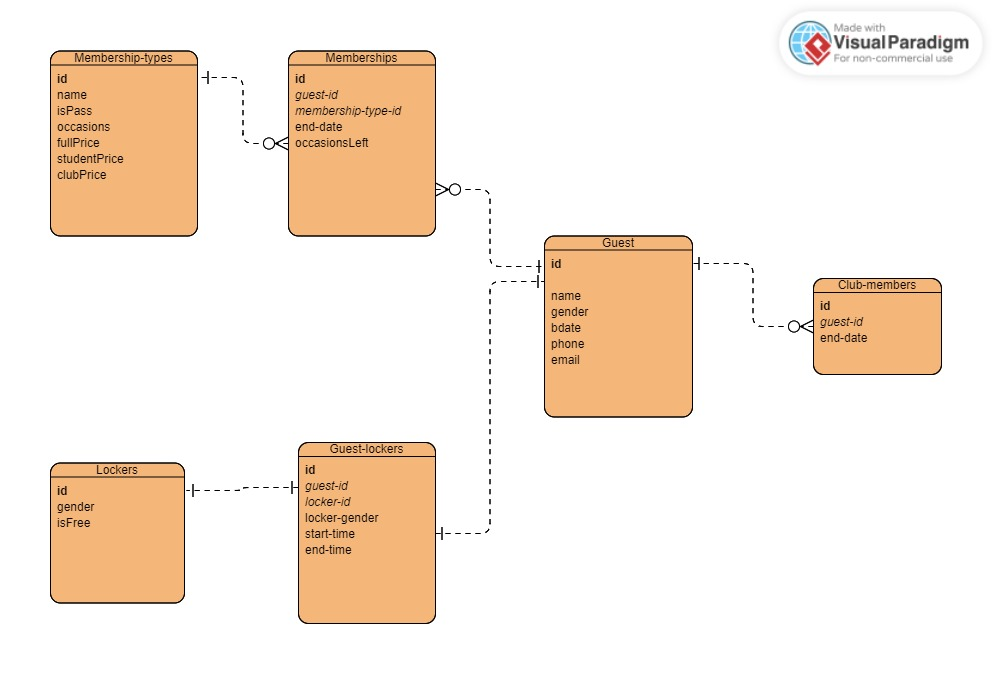
\includegraphics[width=\textwidth]{database}
\caption{A szoftver adatbázis modellje.}
\end{figure}

\begin{figure}
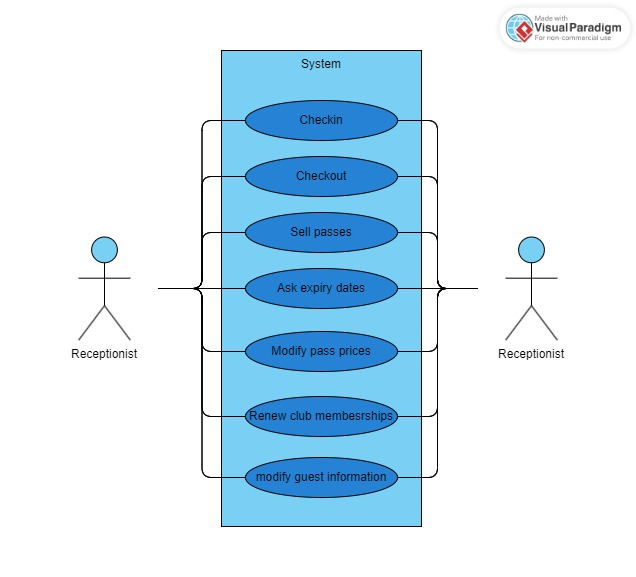
\includegraphics[width=\textwidth]{usecase}
\caption{Használati eset (use case) diagram. }
\end{figure}

\subsection{Implementálás}
\subsection{Tesztelés?}

\subsection{Java Spring backend}

\subsection{A kettő összehasonlítása}

\begin{table}[h!]
\centering
\begin{tabular}{ |p{1.7cm}|p{4.4cm}|p{6.3cm}| } 
\hline
 \textbf{Metódus} & \textbf{Útvonal} &\textbf{Leírás}\\
\hline
GET & /guest/getAll& Az összes vendég lekérése.\\
\hline
GET & /guest/getById/\{id\}& Egy vendég lekérése az azonosítója alapján.\\
\hline
POST & /guest/insertGuest&  Egy új vendég hozzáadása. \\
\hline
PUT & /guest/updateGuest/\{id\} & Egy vendég kartonjának szerkesztése \\
\hline
DELETE & /guest/deleteGuest/\{id\} & Egy vendég törlése  \\
\hline
... & ... &...  \\
\hline
\end{tabular}
\caption{A kérések listájának részlete.}
\end{table}

\newpage
\section*{Összefoglalás}
\addcontentsline{toc}{section}{Összefoglalás}

%******************példa képek:

%\begin{figure}
%\centering
%\includegraphics[width=0.7\textwidth]{org}
%\caption{Organogram.}
%\end{figure}

%\begin{wrapfigure}{r}{0.4\textwidth}
%\includegraphics[width=0.4\textwidth]{test1}
%\caption{Értékteremtő lánc diagram.}
%\end{wrapfigure}

%\begin{figure}[h]
%\centering
%\begin{subfigure}{0.45\textwidth}
%\includegraphics[width=8cm]{pelda1} 
%\end{subfigure}
%\begin{subfigure}{0.4\textwidth}
%\includegraphics[width=8cm]{pelda2}
%\end{subfigure}
%\caption{A háló $t_1$ tüzelése előtt és után}
%\end{figure}

%******************felsorolas
%\begin{definíció}
%A Petri háló ($PN$) egy ($P, T, E, w, m_0$) rendszer, ahol
%\begin{enumerate}
%\item $P$ a helyek véges halmaza,
%\item $T$ a tranzíciók véges halmaza feltéve, hogy $P \cap T = \emptyset$,
%\item $E \subseteq (P \times T) \cup (T \times P)$ az élek véges halmaza,
%\item $ w: E\rightarrow N^+$ a súlyfüggvény,
%\item $ m: P\rightarrow N$ a token-eloszlás függvény,
%\item $ m_0$ a kezdeti token eloszlás.
%\end{enumerate}
%A Petri háló struktúrát $(P, T, E, w)$ módon jelöljük. (\textit{Peterson., 1981})
%\end{definíció}

%******************felsorolas
%\begin{itemize}
%\item egy adott időszakban egy vevő mennyit vásárolt?
%\item melyik partnernek mennyi ki nem fizetett, vagy lejárt tartozása van?
%\item egy adott termékből mennyi fogyott adott idő alatt?
%\item ki állított ki egy bizonyos számlát?
%\item kik vannak jelenleg bejelentkezve?
%\item kinek van lejárt tartozása és mennyi?
%\end{itemize}

\addcontentsline{toc}{section}{Irodalomjegyzék}

\newpage
\renewcommand{\refname}{Irodalomjegyzék}
\begin{thebibliography}{99}

\bibitem{CS}
C. Scalfani. Functional Programming Made Easier: A Step-by-Step Guide. 2021.

\bibitem{PE}
P. Freeman. PureScript by Example. 2014 - 2017.
\url{https://book.purescript.org/}

\bibitem{VD}
Dr. Vadász Dénes: Programozási paradigmák, programozási nyelvek (letölthető egyetemi oktatási anyag)
\url{https://web.archive.org/web/20150501083657/http://www.iit.uni-miskolc.hu/iitweb/export/sites/default/users/DVadasz/GEIAL401/Progpar-4-fejezet.pdf#}
Hozzáférés dátuma: 2023.04.11.

\bibitem{JM}
John McCarthy: The implementation of LISP. 1996.
http://www-formal.stanford.edu/jmc/history/lisp/node3.html

\bibitem{Sz}
Szuromi Zs.: Programozási paradigmák, kézirat. ME, 1996.

\bibitem{TIO}
The TIOBE Programming Community index. \url{https://www.tiobe.com/tiobe-index/} Hozzáférés dátuma: 2023.04.11.

\bibitem{Java}
A Java nyelv hivatalos honlapja. \url{https://dev.java/learn/lambdas/}  Hozzáférés dátuma: 2023.04.11.

\bibitem{sy}
B. Radojicic.: Imperative to Functional Programming in Java. 2022
\url{https://symphony.is/blog/imperative-to-functional-programming-in-java} Hozzáférés dátuma: 2023.04.11.

\bibitem{JN}
J. Neumann.: Advantages and disadvantages of functional programming. 2022.
\url{https://medium.com/twodigits/advantages-and-disadvantages-of-functional-programming-52a81c8bf446}
Hozzáférés dátuma: 2023.04.12.

\bibitem{PS}
\url{https://www.purescript.org/}

\bibitem{vue}
\url{https://vuejs.org/guide/introduction.html}

\bibitem{py}
J. Sturtz.: Functional Programming in Python: When and How to Use It. Hozzáférés dátuma: 2023.04.20.
\url{https://realpython.com/python-functional-programming/}

\bibitem{cpp}
D. Cravey.: Functional-Style Programming in C++. Hozzáférés dátuma: 2023.04.20.
\url{https://learn.microsoft.com/en-us/archive/msdn-magazine/2012/august/c-functional-style-programming-in-c}

\href{https://learn.microsoft.com/en-us/archive/msdn-magazine/2012/august/c-functional-style-programming-in-c}{D. Cravey.: Functional-Style Programming in C++}.\\ Hozzáférés dátuma: 2023.04.20.

\end{thebibliography}
\end{document}
